\documentclass[10pt, a4paper]{scrreprt}

	% TODO: export in Layout-File
	% parse into new layout!
	% create table of bibliography
	% Schriftgröße, Seitenränder, Abstand erhöhen --> erst zum Schluss ;-)

%% --------------------------- LAYOUT ------------------ %%
\usepackage[T1]{fontenc}
\usepackage[utf8]{inputenc}
\usepackage[ngerman]{babel}
\usepackage{amsmath}
\usepackage{amssymb}
\usepackage{selinput}
\usepackage{setspace}
\usepackage{geometry}
\usepackage{graphicx}

\SelectInputMappings{
 adieresis={ä},
 germandbls={ß},
}
\setlength{\topskip}{\ht\strutbox} % behebt Warnung von geometry
\geometry{paper=a4paper,left=30mm,right=20mm,top=20mm} 
\graphicspath{{pictures/}} % Specifies the directory where pictures are stored

% TODO: \onehalfspacing % Zeilenabstand erhöhen (1.5) 
% Seitenränder erhöhen!


%% ------------------------------------------------------ %%
%% ------------------------ BEGIN ---------------------- %%
%% -------------------------------------------------------%% 

\begin{document}


%% ---------------------------- TITLE ------------------------%%
\begin{titlepage}
\title{Implementierung einer Smartphone-Anwendung zum Austausch verschlüsselter Daten mit einer Cloud}
\maketitle
\end{titlepage}

% Text komplett in der Mitte von der Seite!
\vspace*{\fill}
\begin{center}
“If you think technology can solve your security problems, then you don’t understand the problems and you don’t understand the technology.”
\end{center}
\begin{flushright}
Bruce Schneier
\end{flushright}
\vspace*{\fill}


\tableofcontents

%% -------------------- EINLEITUNG ------------------ %%
\chapter{Einleitung}
% \setcounter{page}{1}
	% TODO: Text über Sicherheit, Privatsphäre, Bedürnisse, Internet, Überwachung, Smartphones ..
"Die Computer- und Internetnutzer in Deutschland setzen seit Bekanntwerden der geheimdienstlichen Abhöraktionen häufiger Verschlüsselungsverfahren ein." %[http://www.bitkom.org/files/documents/BITKOM-Presseinfo_Verschluesselung_18_12_2013_v2\%281\%29.pdf]
Aus der Pressemitteilung der BITKOM geht weiterhin hervor, dass von Juli 2013 auf November 2013 insgesamt 1,1 Millionen mehr Bundesbürger ihre persönlichen Dateien verschlüsseln. Besonders wichtig ist der Aspekt der Sicherheit, wenn es sich bei den Daten um relevante oder firmeninterne Informationen handelt, wie es z. B. am Deutschen Elektronen Synchrotron (DESY) in Hamburg der Fall ist. Auch der Austausch von Daten von mobilen Endgeräten wie Smartphones oder Tables spielen eine immer größere Rolle wie die Entwicklung der letzten Jahre zeigt (siehe Grafik). \\ 
\begin{center}
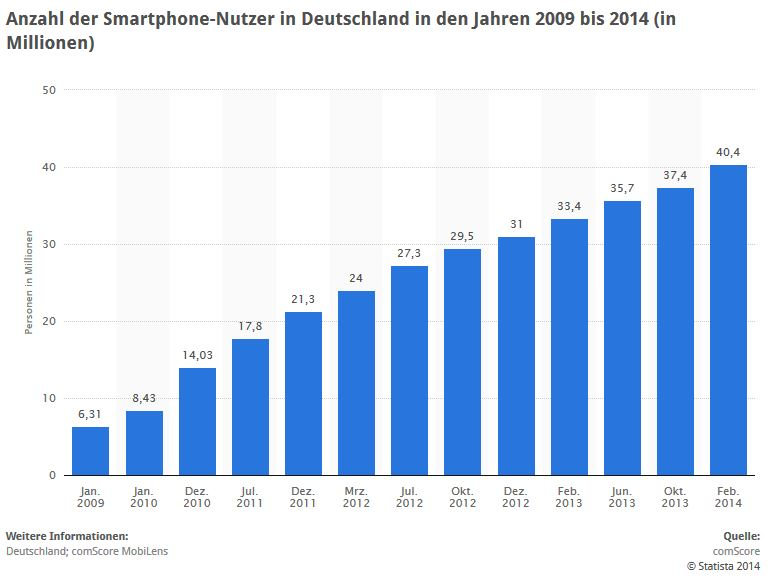
\includegraphics[scale=0.6]{smartphoneUser_Germany.JPG} %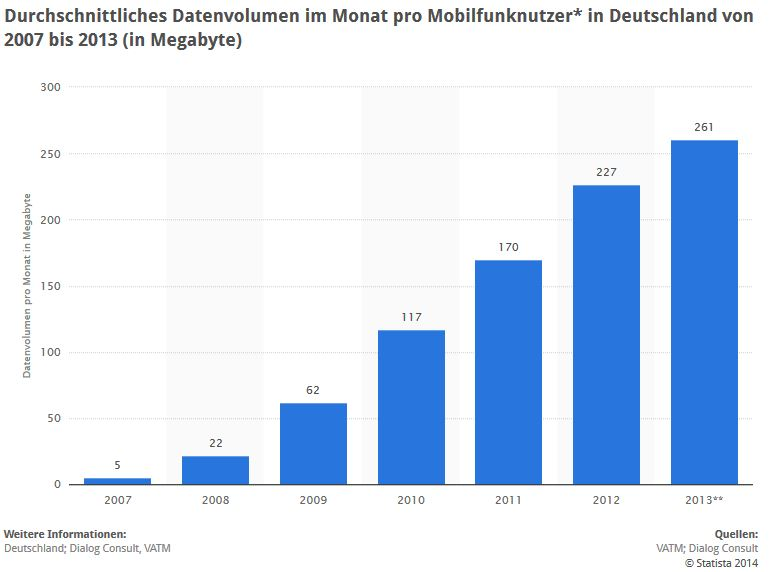
\includegraphics[scale=0.40]{datatraffic_germany.JPG} % zweite Grafik evtl. an anderer Stelle passender?
\end{center}
Herkömmliche Verfahren zum Austausch von Daten reichen oftmals nicht mehr aus, wenn man den Aspekt der Sicherheit näher beleuchtet. % TODO: prüfen? kann man das so stehen lassen?!?


\section{Motivation}
Am Deutschen Elektronen Synchrotron, im folgenden DESY, werden bisher wichtige und sensible Dokumente über ein Programm Namens Dropbox gesichert und verwaltet. Dropbox bietet eine plattformunabhänginge Möglichkeit Dokuente Online abzuspeichern und von einem anderen Standort über ein internetfähiges Gerät wieder zu öffnen [https://www.dropbox.com/]. Auch wenn Dropbox nach eigenen Angaben den Advanced Encryption Standard (AES)  verwendet, bevor die Daten gespeichert werden, liegen die dafür notwendigen Schlüssel in Händen der Betreiber selbst, die somit vollen Klartextzugriff auf die Nutzerdateien haben. Dropbox begründet diesen Zugriff wie folgt:  "Wie die meisten Online-Dienste verfügt auch Dropbox über einen kleinen Mitarbeiterstamm, dem aus in unserer Datenschutzrichtlinie dargelegten Gründen Zugriffsrechte auf Nutzerdaten gewährt werden muss [...]". \\ % TODO [https://www.dropbox.com/help/27/de aufgerufen 01.07.2014]
Da das DESY über eine eigene Cloud-Infrastruktur verfügt, sollen in Zukunft alle wichtigen Daten nicht nur in dieser Cloud gespeichert werden, sondern auch zusätzlich durch eine Verschlüsselung gesichert werden.


\section{Zielsetzung}
Ziel dieser Arbeit ist es aus diesem Grund einen Prototyp zu entwickeln, der einerseits mit dem Cloud-System des DESY Kommunizieren kann um dort Dateien hoch- und herunter zu laden, andererseits diese Daten auch in angemessener Form (siehe Kapitel Validierung) zu Verschlüsseln. \\
In der ersten Version dieser Arbeit wird ein Programm entwickelt, welches auf Android-Betriebssystemen zum Einsatz kommen kann. Darüber hinaus ist es wichtig, dass die entsprechenden Schlüssel zum entschlüsseln der Daten nicht zusammen mit den Daten abgelegt werden, sondern ausschließlich den Parteien des Datenaustauschs bekannt sein soll. Dies bedeutet, das selbst die Betreiber am DESY nicht die Möglichkeit haben die abgelegten Daten zu entschlüsseln. \\
Zum ver- und entschüsseln der Daten sollen Verfahren verwendet werden, die in der heutigen Zeit als sicher angesehen werden und Smartphones im Bezug auf Performance und Akkuverbrauch nicht zu stark belasten. Um diese Faktoren zu Validieren wird eine Testanwendung geschrieben, die mit bestimmten Faktoren die verschiedenen Verfahren untereinander überprüfen (siehe Kapitel Validierung).

	% TODO: Prüfen, ob dieser Part wirklich hier rein muss? Andere Software vergleichen?
\section{Verwandte Arbeiten}
	% TODO: Recherche?!? --> wird nicht benötigt, da es sich bei der Arbeit hautpsächlich um die Entwicklung des Programmes handelt. Kryptographische Verfahren wurdne zu genüge behandelt.
\section{Verwandte Programme}
	% TODO: Unterscheidung in Arbeiten & Programme notwendig?
	% vgl. Dropbox
	% vgl. ownCloud <<- speziell: soll in Zukunft am DESY verwendet werden --> kompatiblität beachten?!? 
	% vgl. boxcryptor
	% vgl. cloudfogger


\section{Diese Arbeit}
\subsection{Inhaltlicher Aufbau}

% \chapter{Anforderungen} ?


%% ---------------------- GRUNDLAGEN ----------------- %%
\chapter{Grundlagen Allgemein}
\section{Cloud}
\section{Kryptografische Definitionen}
	% TODO: anders aufteilen!


\chapter{Grundlagen Android}
In diesem Kapitel wird kurz darauf eingegangen, welche Kryptografischen Aspekte Android in den verschiedenen Versionen zur Verfügung stellt um diese im darauffolgendan Kapitel genauer zu Untersuchen. Aufgrund der Aussage, dass die Android Version Gingerbread (2.3.3) im Juni 2014 noch einen Marktanteil von knapp 15\% hält, ist dies auch die niedrigste vom Programm unterstützte Verstion. \\
\begin{center}
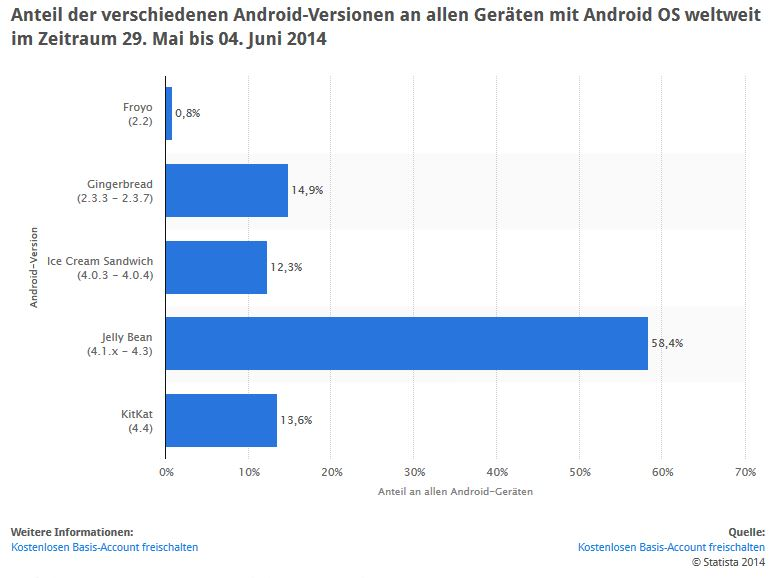
\includegraphics[scale=0.6]{android_version_marktanteil.JPG} %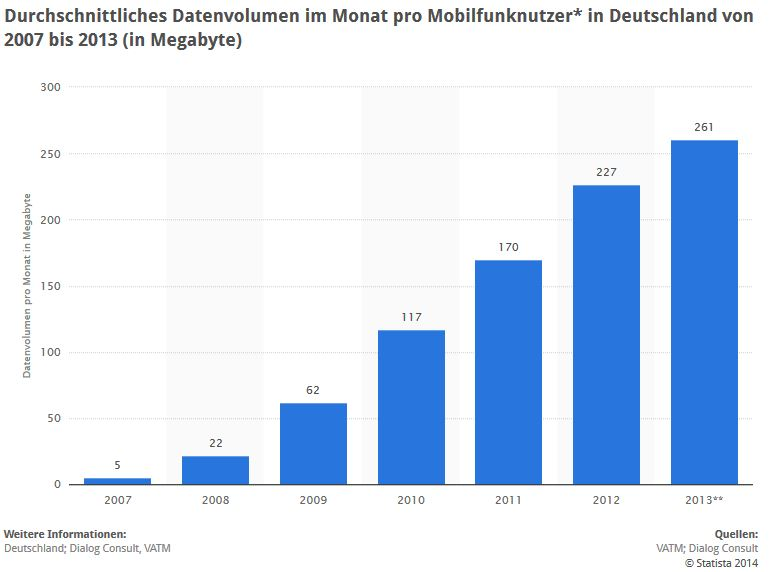
\includegraphics[scale=0.40]{datatraffic_germany.JPG} % zweite Grafik evtl. an anderer Stelle passender?
\end{center}
Bei der Analyse wird darauf geachtet, dass alle Funktionalitäten die im Programm entwickelt werden, von dieser Version unterstützt werden. Die, während des Schreibens dieser Arbeit, aktuellste Version der Android API ist KitKat (4.4), bei der darauf geachtet wird, dass die in von Gingerbread genutzten Funktionen auch in dieser Version noch zur Verfügung stehen und nicht mit \textit{deprecated (veraltet)} markiert sind.


\section{Zusammenhang Kryptographie}
Android stellt mich dem Paket javax.crypto eine Schnittstelle zur Verfügung, mit dem der Programmierer die Möglichkeit hat verschiedene Kryptografische Verfahren aufzurufen, ohne die genaue Implementierung kennen zu müssen. Des Weiteren ist die Klasse abstrahiert von der darunter liegenden Umsetzung der Verfahren. %TODO: Quelle?
In den tieferen Ebenen der Implementierung existieren verschiedene Provider, welche dann die einzelnen Implementierungen der Verfahren zur Verfügung stellen. Mit folgendem Codeabschnitt ist es möglich die einzelnen Provider mit den unterstützten Verfahren auszulesen. \\
\begin{center}
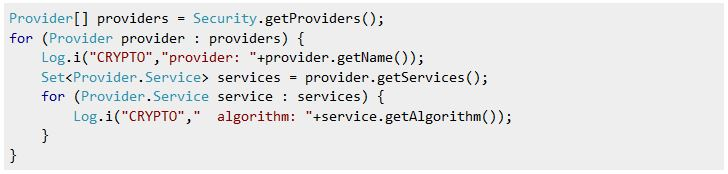
\includegraphics[scale=1.0]{read_cryptoprovider.JPG} %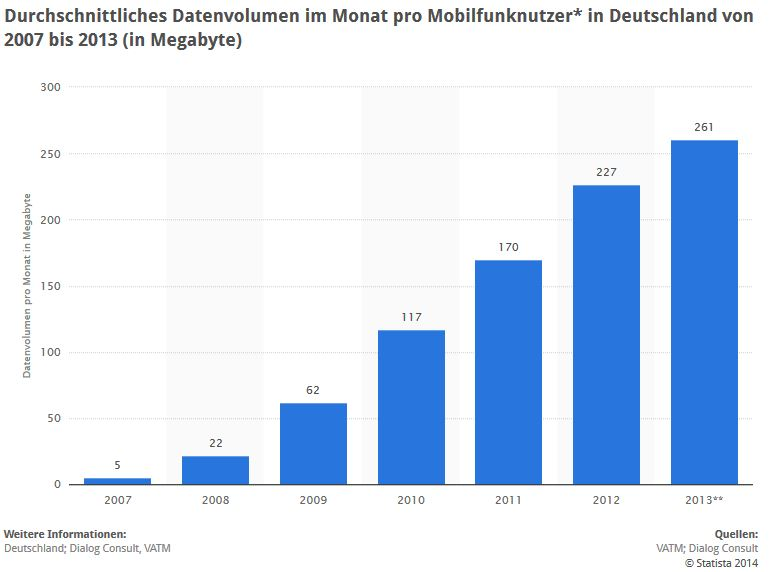
\includegraphics[scale=0.40]{datatraffic_germany.JPG} % zweite Grafik evtl. an anderer Stelle passender?
\end{center}


\section{OpenSSL}
	%TODO: Größere Probleme der letzten Zeit: Heartbleed -> Android 4.1.1 infected
	% eigenständiges Updaten der ossl-version.
	% 
\section{Bouncy Castle}

\chapter{Grundlagen Kryptographie}
	% TODO: Begriffserklärung: integrität, authentifizierung, autorisierung usw. ..
	% tiefe Beschreibung der einzelnen Dinge notwendig?
	% TODO: Ziele, Begriffserklärung: kryptographie, kryptoanalsyse, kryptologie, symetrisch, asymetrisch, 
\section{Verschlüsselung}
\subsection{Symetrische Verfahren}
\subsection{Asymetrische Verfahren}

\section{Hash-Funktionen}
\section{Digitale Signature}
\subsection{Public Key Infrastruktur}
\section{Schlüsselvereinbarung}
\subsection{Diffie Hellmann}
\subsection{ElGamal}
\section{Schlüsselgenerierung}
\section{Authentifizierung}
\subsection{Zwei-Faktor-Authentifizierung}
	% TODO: Erklärung: http://de.wikipedia.org/wiki/Zwei-Faktor-Authentifizierung (need Quelle)


%% ------------------------ VALIDIERUNG --------------------- %%
\chapter{Validierung}
	% TODO: Erläuterung des Testgerätes & der Punkte auf die getestet werden soll!
	% aufzeigen der Notwendigkeit dieser Validierung
\section{Verschlüsselungsverfahren}
\section{Hashfunktionen}

%% ------------------------ IMPLEMENTIERUNG ---------------- %%
\chapter{Implementierung}
\section{Entwurf}

%% ----------------------------- TEST -------------------------- %%
\chapter{Test}
\section{Validierung}
\section{Testverfahren}

%% -------------------------- ZUSAMMENFASSUNG -------------- %%
\chapter{Zusammenfassung und Ausblick}
\section{Zusammenfassung}
\section{Ausblick}

%--------------------------------------------------------------------
% -----------------------ENDE ------------------------------------
%------------------------------------------------------------------


%% --------------------------- BIBLIO --------------------------------%%
%\label{Bibliography}

%\lhead{\emph{Bibliography}} % Change the page header to say "Bibliography"

%\bibliographystyle{unsrtnat} % Use the "unsrtnat" BibTeX style for formatting the Bibliography

%\bibliography{Bibliography} % The references (bibliography) information are stored in the file named "Bibliography.bib"


%Glossar
%Literatur
%Diagramme
%Tabellen
%eigenständigkeitsverklärung

\end{document}